\section{Machine learning algorithms}
In this thesis, we will test our metamorphic relations by using them to generate follow-up test data for machine learning algorithms and checking if the metamorphic properties hold after multiple executions of the system. Thus, we investigated the following common machine learning algorithms. Just like in "Automated Metamorphic System Testing" proposed by Murphy et al. \cite{Murphy2009}, the algorithms we implement are also considered as a black box instead of a white box.
\subsection{Neural network}
Neural networks were first introduced in 1944 by two University of Chicago researchers Warren McCullough and Walter Pitts. The neural network algorithms are modeled loosely after the human brain, which is very efficient in pattern recognition.  Dr. Robert Hecht-Nielsen, who also invented the first neurocomputer, defines a neural network as:
"...a computing system made up of a number of simple, highly interconnected processing elements, which process information by their dynamic state response to external inputs"\cite{Caudill}.
\begin{figure}[htb!]
    \centering
    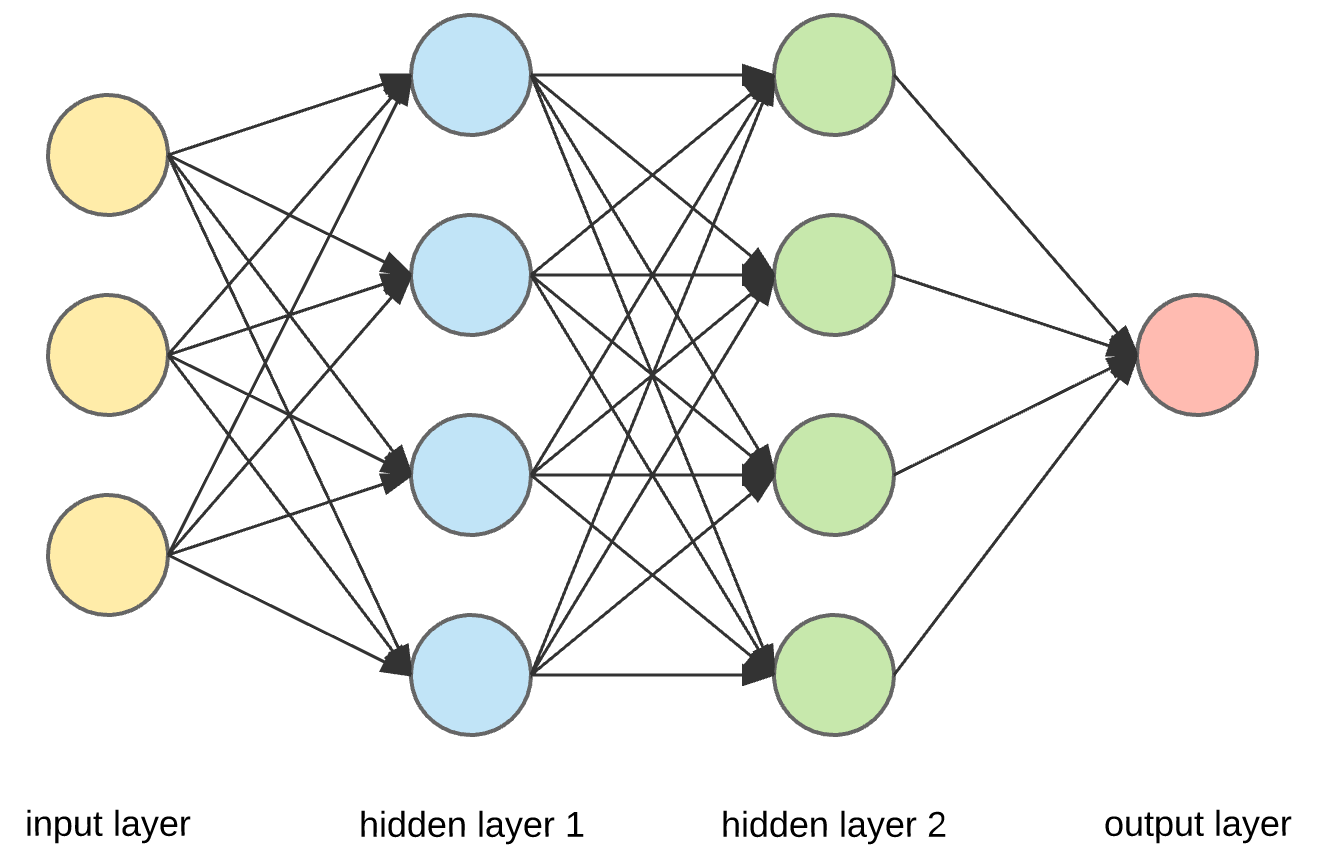
\includegraphics[scale=0.15]{files/nn.png}
    \caption{Neural network}
    \label{Neural network}
    \end{figure}
    \FloatBarrier
% cite figure: https://towardsdatascience.com/applied-deep-learning-part-1-artificial-neural-networks-d7834f67a4f6
A typical neural network looks like a variation of Figure \ref{Neural network} and is composed of the following layers. \\
Input layer: This is the leftmost layer in the network. It is made up of input neurons, and the layer is called the input layer. There is no computation performed in the nodes at this layer. The input layer simply provides information from the environment to the next layer. \\
Hidden layers: The layers in the middle make up the hidden layers. As the name suggests, these layers are neither inputs nor outputs. There can be zero or multiple hidden layers. Hidden layers take the input from the input layer and pass the information to the output or other hidden layer after performing computation on the data. \\
Output layer: The last layer in the neural network is called the output layer. This layer contains the output neurons, which tells the final class of the input. In the example above, we have a single output neuron. \\

% There are no set rules to design the layers of a neural network (specially the hidden layers) and this process is often considered as an art\cite{NN}. The number of hidden layers and nodes are often determined empirically for each particular case in order to optimize performance. The edges (or connections) between a layer and the layer before it are represented by a weight $\omega_{ij}$, which represents the strength of connection between i and j nodes. During the training phase of the neural network, we assign random values to the weights for each connection. The algorithm then tries to optimize the weights so that the error function is minimized. For each node at a layer all the output from the previous node is multiplied by the weight of connections between them and the sum of all the different connections produces the value at that node. This cycle is repeated for all the nodes in every layer. The algorithm compares the prediction from the output layer to the real value and readjusts the weights. Once the optimal value is reached the network can be used to make predictions\cite{hall199}.
There are no set rules to design the layers of a neural network (especially the hidden layers), and this process is often considered as an art\cite{NN}. The number of hidden layers and nodes is often determined empirically for each particular case in order to optimize performance. The edges (or connections) between two layers($i$ and $j$) are represented by weight $\omega_{ij}$, which represents the strength of the connection between $i$ and $j$ nodes. When the neural network is being trained, we assign random values to the weights for each connection. The weights are then optimized such that the error function is minimized. For each node at a layer, all the outputs from the previous nodes are multiplied by the weight of connections between them. The weighted outputs are then summed and used as the value at that node. This cycle is repeated for all the nodes in every layer. The algorithm compares the prediction from the output layer to the real value and readjusts the weights. Once the optimal value is reached, the network can be used to make predictions\cite{hall199}.

These neural networks where the input of a layer is received from the output of the previous layer are called feedforward neural networks\cite{NN}\cite{hall199}. The feedforward neural network has no loops, and the information flows in one direction and is never fed back. The most well-known form of a feedforward neural network is called a multilayer perceptron(MLP). MLPs are also called universal function approximator. An MLP with one hidden layer and a sufficient number of nonlinear units can act as a continuous function on a narrow input domain with arbitrary precision \cite{Graves}.
Other models of artificial neural networks where a feedback loop is possible are called recurrent neural networks. The neurons in these networks fire for a limited duration of time before becoming dormant. However, the firing stimulates other neurons in the network, which may fire after some time for a limited duration of time. This can have a cascading effect causing yet other neurons to fire later. Having loops in these models does not create problems since the neurons firing does not affect their input instantly but at a later time. Even though the recurrent neural networks are much similar to our brains than feedforward networks, they have not been as influential as the feedforward networks. This is mostly because the learning algorithms for recurrent nets are (at least to date) less powerful than feedforward networks. In the future, it will be possible that the recurrent networks will be able to solve significant problems which feedforward networks solve with great difficulty.\cite{NN}
% cite: http://neuralnetworksanddeeplearning.com/chap1.html



\subsection{Convolutional neural network}
% Convolutional neural networks (ConvNet) are very similar to ordinary neural networks in structure. They work by extracting simple features at a higher resolution and then converting them into more complex features at a coarser resolution \cite{simard2003best}. It does so by performing dot product on the inputs received at each neuron and optionally follow it with non-linearity. Just like a normal neural network, convolutional neural network (from the input image to output class) can be expressed as a single differential function. It also has a loss function on the fully-connected output layer and the neurons have learnable weights and biases which are optimized during the learning phase.

% What makes it different from an ordinary neural network is the architecture of a ConvNet. It makes explicit assumption that the inputs are images, which allows us to encode certain properties into the architecture. In particular, unlike a regular Neural Network, the layers of a ConvNet have neurons arranged in 3 dimensions: width, height, depth. A simple ConvNet is a sequence of layers and every layer transforms one volume of activation to another through a differentiable function.
Convolutional neural networks (ConvNet) are very similar to the conventional neural networks in terms of structure.  They work by extracting simple features at a higher resolution and transforming them into more complex features at a more granular resolution \cite{simard2003best}. It does so by performing dot product on the inputs received at each neuron and optionally follow it with non-linearity. Just like a typical neural network, ConvNets (from the input image to output class) can be represented with a single differential function. The neurons in ConvNets have learnable weights and biases, which are optimized during the learning phase.  It also has a loss function on the fully-connected output layer, which is minimized.

What makes it different from an ordinary neural network is the architecture of a ConvNet. It makes very specific assumptions that the inputs are images, which allows us to encode specific properties into the architecture. In particular, unlike a regular Neural Network, the neurons in the layers of a ConvNet are arranged in 3 dimensions: width, height, depth. A simple ConvNet is a sequence of layers, and every layer transforms one volume of activation to another through a differentiable function.

\begin{figure}[htb!]
    \centering
    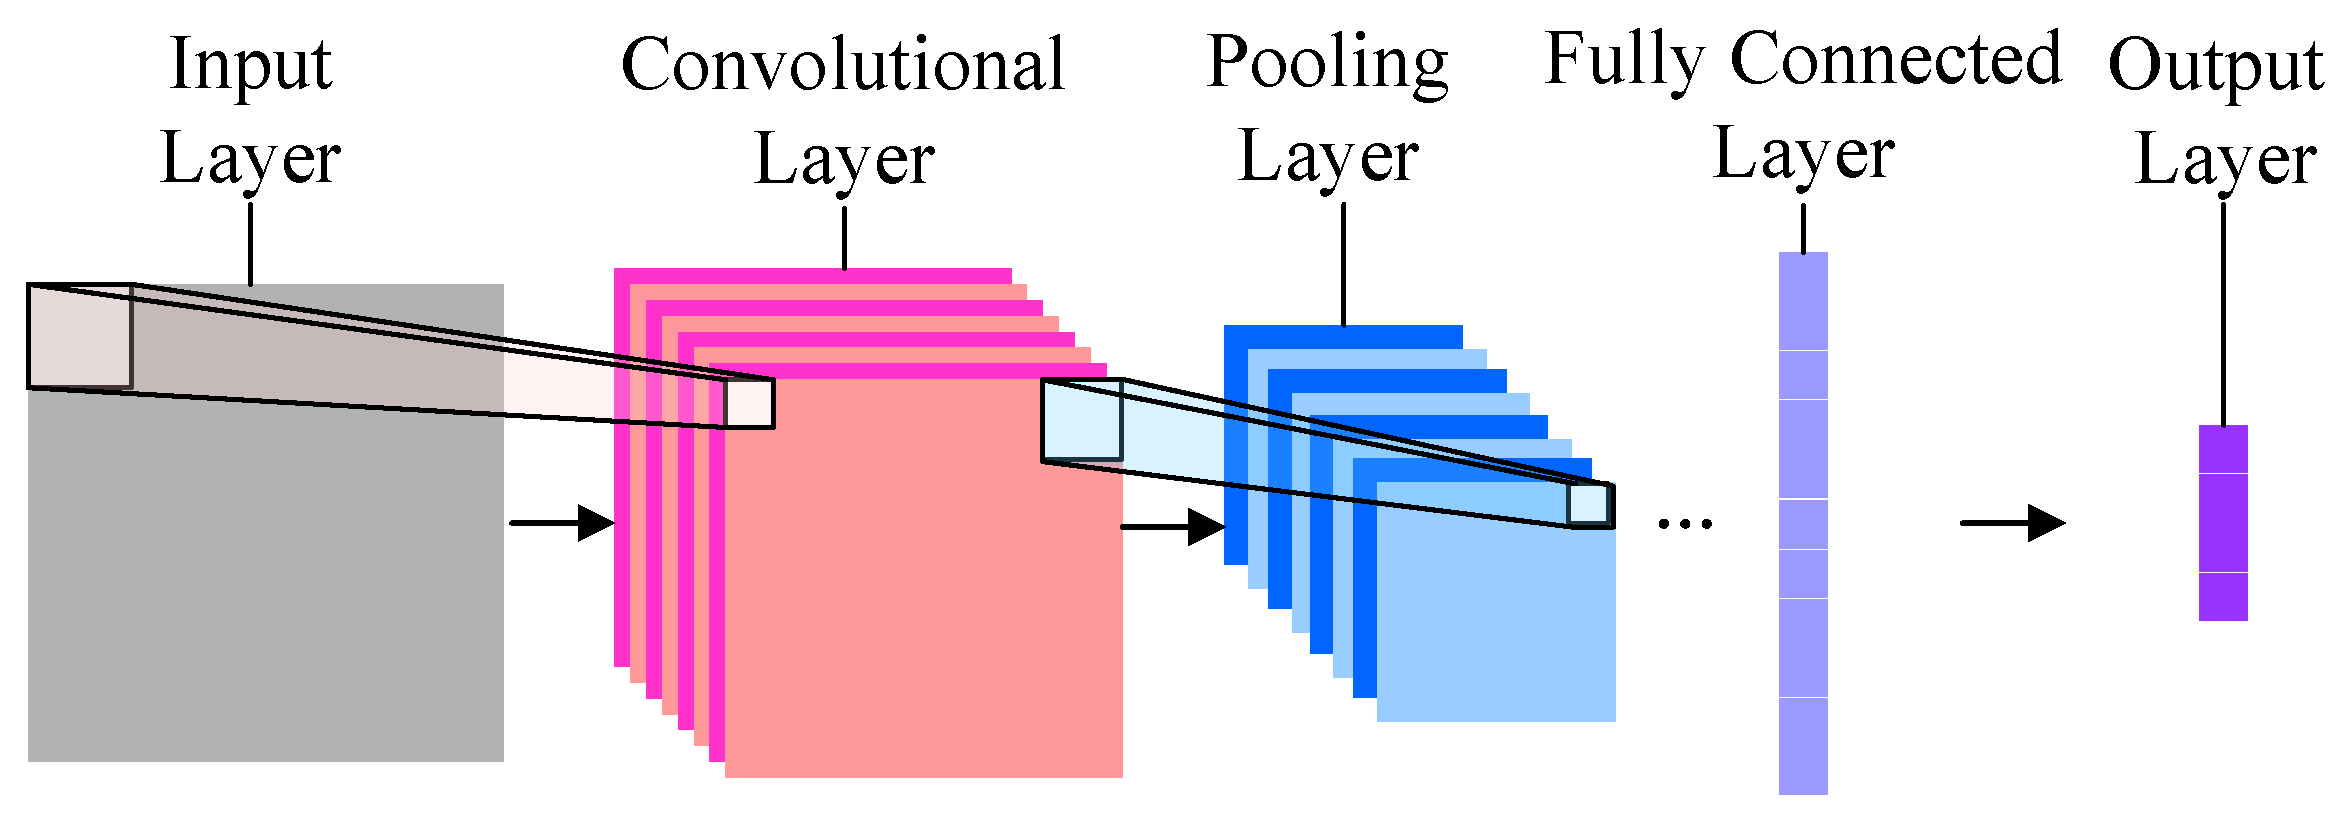
\includegraphics[scale=1.25]{chapters/litReview/files/convNet.png}
    \caption{Convolutional Neural network \cite{convNN}}
    \label{Convolutional Neural network}
    \end{figure}
    \FloatBarrier
    
% A ConvNet architecture is made up of the following layers and these layers are stacked to form the full network \cite{krizhevsky2012imagenet}: \\
% Input layer: This layer holds the raw input image in form of it's pixel values and color channels.\\
% Convolutional layer (Conv): This layer computes the dot product between it's weight and a small region in the previous layer it is connected to. It is a linear operation which multiplies the input from the previous layer to a two-dimensional array of weights called filter or kernel. \\
% Rectified linear unit (ReLu): This layer applies an element-wise activation function, like $max(0,x)$ with the threshold at zero. It introduces non-linearity to the system which has just been doing linear computations (element wise multiplication and sum) in previous Conv layers. \\
% Pooling layer (POOL): This layer performs a downsampling operation along the spatial dimensions. This helps in two major ways: $i)$ The amount of parameters or weights is reduced by 75\%. $ii)$ It also reduces the problem of overfitting.\\
% Fully connected layer (FC): The fully connected output layer computes the class scores for the input. The neurons in this layer are connected to every neuron in the previous layer. The only difference between this layer and the Conv layer is that the neurons in Conv layer are only connected to a local region in the input layer and the neurons in Conv layer share parameters. The neurons in both the layer compute dot product and their function form is identical. Thus, it is easily possible to convert between the fully connected and Conv layer.\\
A ConvNet architecture is made up of the following layers. The full network is made of multiple instances of these layers stacked one after other \cite{krizhevsky2012imagenet}: \\
Input layer: This layer contains the raw input image in the form of its pixel values and color channels.\\
Convolutional layer (Conv): This layer calculates a dot product between its assigned weights and a small region in the previous layer it is connected to. It is a linear operation that multiplies the input from the previous layer to a two-dimensional array of weights called filter or kernel. \\
Rectified linear unit (ReLu): This layer applies an element-wise activation function, like $max(0,x)$ with the threshold at zero. The purpose of this layer is to introduce non-linearity to a system, which has just been doing linear computations (element-wise multiplication and sum) so far. \\
Pooling layer (POOL): This layer performs a downsampling operation along the spatial dimensions. This helps in two major ways: $i)$ The amount of parameters or weights is reduced by 75\%. $ii)$ It also reduces the problem of overfitting.\\
Fully connected layer (FC): The fully connected output layer is used to compute the class scores for an input. The only difference between this layer and the Conv layer is that the neurons in the Conv layer are only connected to a local region in the input layer while the neurons in the FC layer are connected to every neuron in the previous layer. The neurons in both the layer compute dot product, and their function form is identical. Thus, it is easily possible to convert between the fully connected and Conv layer.

It should be noted that some layers have parameters, while others may not. The ReLu/Pool layer implements a fixed function, whereas the Conv/FC layers transformation functions work on the activations in the input volume and the parameters (weights and biases) of the neurons. During the training period, the weights and biases of the Conv/FC layer are trained using gradient descent. The parameters are trained such that the scores computed by ConvNet generate outputs that match the expected output of each image in the training set \cite{convNNStan}.
% It should be noted that some layers contain parameters while others may not. The ReLu/Pool layer implements a fixed function whereas, the Conv/FC layers transformation functions work on the activations in the input volume and the weights and biases of the neurons. The parameters in Conv/FC layer is trained using gradient descent such that the scores computed by ConvNet is consistent with the expected output of each image in the training set \cite{convNNStan}.
%cite http://cs231n.github.io/convolutional-networks/

\subsection{Naive Bayes}
% In it's simplest form a Naive Bayes algorithm is a type of Bayesian network where all attributes are independent given the value of the class variable. This property is called conditional independence. It is obvious that the conditional independence assumption is rarely true in most real-world applications\cite{zhang2004optimality}. Despite this limitation the algorithm is very popular and works quite well in many real-world situations like document classification and spam filtering. The classifier is a really common supervised learning algorithm because it is fast, easy to implement and relatively effective. They also require relatively small number of training data to estimate the necessary parameters of the network\cite{scikit-learn}. Given a class variable $y$ and dependent feature vector $x_{1}$...$x_{n}$, Bayes theorem states that:
In its purest form, a Naive Bayes algorithm is a type of Bayesian network. Naive Bayes algorithm is conditionally independent, i.e., the attributes of the data are independent, given the value of classes. However, the data is rarely conditionally independent in most real-world problems\cite{zhang2004optimality}. Even with these limitations, the Naive Bayes algorithms fare well in most real-world problems like spam filtering and document classification. Due to its speed, effectiveness, and simplicity, Naive Bayes is a very common learning algorithm. The number of training data required to train the parameters of the network is also relatively small \cite{scikit-learn}. \\
Bayes theorem states that:
\begin{center}
    $P(y|x_{1},...,x_{n}) = \frac{P(y)P(x_{1},...,x_{n}|y)}{P(x_{1},...,x_{n})}$\\
    where $y$ is the class variable and $x_1,\dots,x_n$, are the dependent feature vectors.
\end{center}
\begin{center}
Since the features in Naive Bayes are independent: 
$P(y \mid x_1, \dots, x_n) = \frac{P(y) \prod_{i=1}^{n} P(x_i \mid y)}
                                 {P(x_1, \dots, x_n)}$
\end{center}
% Include the equations from https://scikit-learn.org/stable/modules/naive_bayes.html
For a given input we know that $P(x_{1},...,x_{n})$ is constant. Therefore: 
\begin{center}
$P(y \mid x_1, \dots, x_n) \propto P(y) \prod_{i=1}^{n} P(x_i \mid y)$
\end{center}
And an expected classification $\hat{y}$ can be obtained by finding the value of $y$ such that $P(y \mid x_1, \dots, x_n)$ is maximized:
\begin{center}
$\hat{y} = \arg\max_y P(y) \prod_{i=1}^{n} P(x_i \mid y)$
\end{center}
% The main distinction between different versions of naive Bayes classifiers are the assumptions they make about the distribution of $P(x_i \mid y)$\cite{scikit-learn}. The multinomial Naive Bayes suffers from a systematic problem of assigning poor weights to necessary parameters if once class has more training examples than others. This effect lowers the weights for classes with less training examples\cite{rennie2003tackling}. For this reason we have equal numbers of training and testing examples for each class in our experiment. 
There are multiple versions of Naive Bayes classifier, but the main distinction between them is the assumptions they make about the distribution of $P(x_i \mid y)$\cite{scikit-learn}. The multinomial Naive Bayes suffers from a systematic problem of assigning poor weights to necessary parameters in an unbalanced training dataset. If one class has fewer training examples than others, the algorithm lowers the weights for thoseclasses\cite{rennie2003tackling}. For this reason, we have equal numbers of training and testing examples for each class in our experiment. 

\subsection{$k$-Nearest Neighbor}
% The nearest neighbor classifier is a supervised classification technique which assigns an input sample vector (whose classification is to be predicted) to the class of it's nearest neighbors. The similarity between the input and the neighbors is calculated based on some distance metrics. This process does not require any pre-processing of the labeled set of neighbors before their use \cite{cover1967}. This idea can be further extended to assign the class of input variable to the class represented by majority of the $k$ nearest neighbors, where $k$ is a positive number specified by the user. The optimal value of $k$ depends on the data. A larger value of $k$ makes the classification boundaries less distinct while suppressing the noise effect \cite{scikit-learn}. One problem with implementing $k$ nearest algorithm is that in some cases there may be a tie among classes between the $k$ neighbors. This problem can be solved by restricting the values of $k$. In a binary classification problem, the values of $k$ can be restricted to odd numbers so that ties can be avoided. In a multi-class classification, this can be resolved by assigning the input to the class for which the sum of distance to each neighbor is the least. This could further lead to a tie and in that case an arbitrary assignment has to be made \cite{keller1985}.
The nearest neighbor classifier is a supervised classification technique that assigns the class of an input vector (whose classification needs to be predicted) to the class of its nearest neighbors. The similarity between the input and the neighbors is calculated based on some distance metrics. This process does not require any pre-processing of the labeled set of neighbors before their use \cite{cover1967}. 
This idea can be further extended to assign the class of an input variable to the class represented by the majority of its $k$ of the nearest neighbors, where $k$ is a positive number specified by the user. 
The optimal value of $k$ depends upon the data. A larger value of $k$ will make the classification boundaries less distinct but suppress the effect of noise \cite{scikit-learn}. One problem with implementing the $k$ nearest algorithm is that in some cases, there may be a tie among classes between the $k$ neighbors. This problem can be solved by restricting the values of $k$. In binary classification problems, the values of $k$ can be restricted to odd numbers so that ties can be avoided. In multi-class classifications, this can be resolved by assigning the input to the class for which the sum of the distance to each neighbor is the least. However, even this could lead to a tie, and in that case, an arbitrary assignment has to be made \cite{keller1985}.

\begin{figure}[htb!]
    \centering
    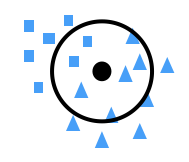
\includegraphics[scale=1]{files/knn.png}
    \caption{$k$-Nearest neighbor: the black dot is assigned to triangle}
    \label{k-Nearest neighbor}
    \end{figure}
    \FloatBarrier


% Given a set of n test data $(x_i, y_i),\dots(x_n, y_n)$ where $x_i$ is the feature vector and $y_i$ is the class label. $x_i$ is defined in a feature space $X$ with distance metric $d$. For a new incoming input $(x, y)$ the goal is to estimate the value of $y$ using the set of already classified data points. A data point $\acute{x_n} \in (x_1, x_2, \dots x_n)$ is said to be the nearest neighbor of $x$ if:
% \begin{center}
% $min\ d(x_i,x) = d(\acute{x_n},x) i = 1,2,3...,n.$ 
% \end{center}
% $x$ is then assigned to the category of $\acute{y_n}$. If $k = 1$, the algorithm assigns $x$ to the category of it's nearest neighbor, ignoring the others. In general, $k$-NN assigns $x$ to the majority class of nearest $k$ neighbors \cite{cover1967}.
Given a set of n classified data $(x_i, y_i),\dots(x_n, y_n)$ where $x_i$ is the feature vector and $y_i$ is their class label. $x_i$ is defined in a feature space $X$ with distance metric $d$. For a new incoming input $(x, y)$ to be classified, the goal is to assign the value of $y$ using the set of already classified data points. A data point $\acute{x_n} \in (x_1, x_2, \dots x_n)$ is said to be the nearest neighbor of $x$ if:
\begin{center}
$min\ d(x_i,x) = d(\acute{x_n},x); for i = 1,\dots,n.$ 
\end{center}
$x$ is then assigned to the category of $\acute{y_n}$. If $k = 1$, the algorithm assigns $x$ to the category of it's nearest neighbor, ignoring the others. If the value of $k$ is more than one then $k$-NN will assign $x$ to the majority class $k$ of its nearest neighbors \cite{cover1967}.

\subsection{Support vector machine}
% A support vector machine (SVM) is a supervised machine learning classifier based on the structural risk minimization (SRM) principal. It solves learning problems by making decision-based rules and minimizing error for independent samples \cite{svm2008}. It has gained rapid popularity in the fields of machine learning, pattern recognition and computer vision because of high accuracy and good generalization capability. SVM creates a decision boundary, also known as hyperplanes, between elements of two classes that allows it to make predictions from one or more feature vectors. The hyperplanes are oriented such that it maximizes the distance between the closest data points in the two classes. These closest points are called support vectors. Support vectors are the input data $x_i$ for which $|y_i|(wx_i^T + b)=1$. It creates these nonlinear boundaries by mapping input vectors to a higher dimensional feature space \cite{SAMANTA2003657,Nakajima2016}.
A support vector machine (SVM) is another type of supervised machine learning classifier, which is based on the principle of structural risk minimization (SRM). 
It works by making decision-based rules and minimizing error for independent samples \cite{svm2008}. It has gained rapid popularity in the fields of machine learning, pattern recognition, and computer vision because of high accuracy and good generalization capability. SVM solves the learning problem by fitting a hyperplane, also known as decision boundary, between elements of two classes that allows it to make predictions from one or more feature vectors. The hyperplanes are oriented such that the distance between the closest data points (also called support vectors) in the two classes is maximum. Support vectors are the input data $x_i$ for which $|y_i|(wx_i^T + b)=1$. It creates these nonlinear boundaries by mapping input vectors to a higher dimensional feature space \cite{SAMANTA2003657,Nakajima2016}.


\begin{figure}[htb!]
    \centering
    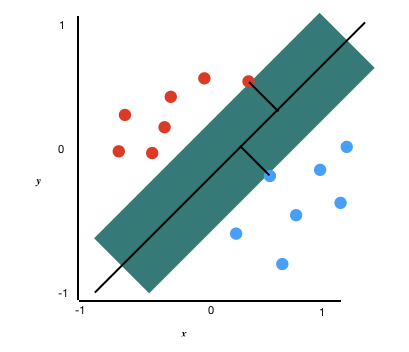
\includegraphics[scale=0.75]{files/svm.png}
    \caption{SVM maximizes the margin between classes}
    \label{SVM maximizes the margin between classes}
    \end{figure}
    \FloatBarrier
    
Given a set of training feature vector $x_i \in R_d$ with label $y_i \in (−1, +1)$: $(x_1, y_1), ..., (x_n, y_n)$ \\
A hyperplane is defined as:
\begin{center}
    $wx^T + b=0$
\end{center}
Where $b$ is the bias, and $w$ is the weight vector. The following conditions should hold for all the elements in the training set:
\begin{center}
    $wx_i^T + b \geq +1$ if $y_i=1$\\
    $wx_i^T + b \leq −1$ if $y_i=–1$
\end{center}
During the training step, the model tries to place the hyperplane such that it maximizes the distance between the support vectors. This is done by finding the optimal values for $w$ and $b$ such the value of $1/(\parallel w\parallel)^2$ is maximum.

    
The obvious problem with SVM described above is that it works only in binary classification problems. A number of methods can be employed to enable SVM for multiclass classification. To classify an input data to three classes, x, y, and, z, three SVMs are needed to answer: $i)$ Is it x? $ii)$ Is it y? $iii)$ Is it z?\cite{noble2006support}.
An alternative way is to make use of kernel methods, which can represent and transform higher dimensional, non-linear models easily. 
% A kernel function helps us to do faster calculations which would otherwise require higher dimensional computation. It adds additional dimension to the input data and makes it a linear problem in a higher dimensional feature space.
A kernel function helps us to do faster calculations which would otherwise require higher dimensional computation. 
It transforms the input data into a higher dimensional linear problem by adding additional dimensions, which can be easily solved in higher dimensional feature space.
A kernel function is defined as:
\begin{center}
  $K (x, y)=<f(x), f(y)>$   
\end{center}
where $K$ is the kernel function, $x, y$ are $m$ dimensional inputs. The function $f$ maps the inputs from $m$ dimensional feature space to $n$ dimensional feature space and
$<x, y>$ denotes a dot product.\\
% Kernels can heavily affect the performance of a SVM but unfortunately there is no set way of choosing a kernel. We can start with a simpler kernel and then experiment with a number of standard kernels to produce best predictions by using cross-validation \cite{huang2018applications}.
Kernels can profoundly affect the performance of an SVM. Unfortunately, there is no fixed strategy to pick a kernel. The best strategy to select a kernel is by starting with a simpler kernel and then experiment with standard kernels, and select the one which produces the best predictions \cite{huang2018applications}.

